
%(BEGIN_QUESTION)
% Copyright 2014, Tony R. Kuphaldt, released under the Creative Commons Attribution License (v 1.0)
% This means you may do almost anything with this work of mine, so long as you give me proper credit

Due to the effects of a changing electric field on the dielectric of a capacitor, some energy is dissipated in capacitors subjected to AC.  Generally, this is not very much, but it is there.  This dissipative behavior is typically modeled as a series-connected resistance:

$$\includegraphics[width=15.5cm]{i01050x01.eps}$$

Calculate the magnitude and phase shift of the current through this capacitor, taking into consideration its equivalent series resistance (ESR):

$$\includegraphics[width=15.5cm]{i01050x02.eps}$$

Compare this against the magnitude and phase shift of the current for an ideal 0.22 $\mu$F capacitor.

\underbar{file i01050}
%(END_QUESTION)





%(BEGIN_ANSWER)

${\bf I} =$ 3.732206 mA $\angle$ 89.89$^{o}$ for the real capacitor with ESR.

\vskip 10pt

${\bf I} =$ 3.732212 mA $\angle$ 90.00$^{o}$ for the ideal capacitor.

%(END_ANSWER)





%(BEGIN_NOTES)

Although capacitors do contain their own parasitic effects, ESR being one of them, they still tend to be much ``purer'' components than inductors for general use.  This is another reason why capacitors are generally favored over inductors in applications where either will suffice.

%INDEX% Electronics review: AC reactance and impedance

%(END_NOTES)


